\documentclass[12pt, a4paper, oneside]{ctexart}
\usepackage{amsmath, amsthm, amssymb, bm, color, graphicx, geometry, mathrsfs,extarrows, braket, booktabs, array, xcolor, fontspec, appendix, float, subfigure, wrapfig, enumitem, titlesec}
\usepackage[colorlinks,linkcolor=red,anchorcolor=blue,citecolor=blue,urlcolor=blue,menucolor=black]{hyperref}

%%%% 设置中文字体 %%%%
% fc-list -f "%{family}\n" :lang=zh >d:zhfont.txt 命令查看已有字体
\setCJKmainfont[
    BoldFont=方正黑体_GBK,  % 黑体
    ItalicFont=方正楷体_GBK,  % 楷体
    BoldItalicFont=方正粗楷简体,  % 粗楷体
    Mapping = fullwidth-stop  % 将中文句号“.”全部转化为英文句号“.”,
]{方正书宋简体}  % !!! 注意在Windows中运行请改为“方正书宋简体.ttf” !!!
%%%% 设置英文字体 %%%%
\setmainfont{Minion Pro}
\setsansfont{Calibri}
\setmonofont{Consolas}

%%%% 设置代码块 %%%%
% 在vscode中使用minted需要先配置python解释器, Ctrl+Shift+P, 输入Python: Select Interpreter选择安装了Pygments的Python版本. 再在setting.json中xelatex和pdflatex的参数中加入 "--shell-escape", 即可
% TeXworks中配置方法参考: https://blog.csdn.net/RobertChenGuangzhi/article/details/108140093
\usepackage{minted}
\renewcommand{\theFancyVerbLine}{
    \sffamily\textcolor[rgb]{0.5,0.5,0.5}{\scriptsize\arabic{FancyVerbLine}}} % 修改代码前序号大小
% 加入不同语言的代码块
\newmintinline{cpp}{fontsize=\small, linenos, breaklines, frame=lines}
\newminted{cpp}{fontsize=\small, baselinestretch=1, linenos, breaklines, frame=lines}
\newmintedfile{cpp}{fontsize=\small, baselinestretch=1, linenos, breaklines, frame=lines}
\newmintinline{matlab}{fontsize=\small, linenos, breaklines, frame=lines}
\newminted{matlab}{fontsize=\small, baselinestretch=1, mathescape, linenos, breaklines, frame=lines}
\newmintedfile{matlab}{fontsize=\small, baselinestretch=1, linenos, breaklines, frame=lines}
\newmintinline{python}{fontsize=\small, linenos, breaklines, frame=lines, python3}  % 使用\pythoninline{代码}
\newminted{python}{fontsize=\small, baselinestretch=1, linenos, breaklines, frame=lines, python3}  % 使用\begin{pythoncode}代码\end{pythoncode}
\newmintedfile{python}{fontsize=\small, baselinestretch=1, linenos, breaklines, frame=lines, python3}  % 使用\pythonfile{代码地址}

%%%% 设置行间距与页边距 %%%%
\linespread{1.3}
\geometry{left=2.5cm, right=2.5cm, top=2.5cm, bottom=2.5cm}
% \geometry{left=1.84cm,right=1.84cm,top=2.18cm,bottom=2.18cm}  % 更小的页边距

%%%% 定理类环境的定义 %%%%
\newtheorem{example}{例}            % 整体编号
\newtheorem{theorem}{定理}[section] % 定理按section编号
\newtheorem{definition}{定义}
\newtheorem{axiom}{公理}
\newtheorem{property}{性质}
\newtheorem{proposition}{命题}
\newtheorem{lemma}{引理}
\newtheorem{corollary}{推论}
\newtheorem{condition}{条件}
\newtheorem{conclusion}{结论}
\newtheorem{assumption}{假设}
\numberwithin{equation}{section}  % 公式按section编号 (公式右端的小括号)
\newtheorem{algorithm}{算法}

%%%% 自定义环境 %%%%
\newsavebox{\nameinfo}
\newenvironment{myTitle}[1]{
    \begin{center}
    {\zihao{-2}\bf #1\\}
    \zihao{-4}\it
}{\end{center}}  % \begin{myTitle}{标题内容}作者信息\end{myTitle}
\newcounter{problem}  % 问题序号计数器
\newenvironment{problem}[1][]{\stepcounter{problem}\par\noindent\textbf{题目\arabic{problem}. #1}}{\smallskip\par}
\newenvironment{solution}[1][]{\par\noindent\textbf{#1解答. }}{\smallskip\par}  % 可带一个参数表示题号\begin{solution}{题号}
\newenvironment{note}{\par\noindent\textbf{注记. }}{\smallskip\par}
\newenvironment{remark}{\begin{enumerate}[label=\textbf{注\arabic*.}]}{\end{enumerate}}
\BeforeBeginEnvironment{minted}{\vspace{-0.5cm}}  % 缩小minted环境距上文间距
\AfterEndEnvironment{minted}{\vspace{-0.2cm}}  % 缩小minted环境距下文间距

%%%% 自定义段落开头序号,间距 (titlesec) %%%%
% 中文序号:\zhnum{section}, 阿拉伯序号:\arabic
\titleformat{\section}{\Large\bfseries}{\arabic{section}}{1em}{}[]
\titlespacing{\section}{0pt}{1.2ex plus .0ex minus .0ex}{.6ex plus .0ex}
\titlespacing{\subsection}{0pt}{1.2ex plus .0ex minus .0ex}{.6ex plus .0ex}
\titlespacing{\subsubsection}{0pt}{1.2ex plus .0ex minus .0ex}{.6ex plus .0ex}

%%%% 图片相对路径 %%%%
\graphicspath{{figures/}} % 当前目录下的figures文件夹, {../figures/}则是父目录的figures文件夹
\setlength{\abovecaptionskip}{-0.2cm}  % 缩紧图片标题与图片之间的距离
\setlength{\belowcaptionskip}{0pt} 

%%%% 缩小item,enumerate,description两行间间距 %%%%
\setenumerate[1]{itemsep=0pt,partopsep=0pt,parsep=\parskip,topsep=5pt}
\setitemize[1]{itemsep=0pt,partopsep=0pt,parsep=\parskip,topsep=5pt}
\setdescription{itemsep=0pt,partopsep=0pt,parsep=\parskip,topsep=5pt}

%%%% 自定义公式 %%%%
\everymath{\displaystyle} % 默认全部行间公式, 想要变回行内公式使用\textstyle
\DeclareMathOperator*\uplim{\overline{lim}}     % 定义上极限 \uplim_{}
\DeclareMathOperator*\lowlim{\underline{lim}}   % 定义下极限 \lowlim_{}
\DeclareMathOperator*{\argmax}{arg\,max}  % 定义取最大值的参数 \argmax_{}
\DeclareMathOperator*{\argmin}{arg\,min}  % 定义取最小值的参数 \argmin_{}
\let\leq=\leqslant % 简写小于等于\leq (将全部leq变为leqslant)
\let\geq=\geqslant % 简写大于等于\geq (将全部geq变为geqslant)
\DeclareRobustCommand{\rchi}{{\mathpalette\irchi\relax}}
\newcommand{\irchi}[2]{\raisebox{\depth}{$#1\chi$}} % 使用\rchi将\chi居中

%%%% 一些宏定义 %%%%
\def\bd{\boldsymbol}        % 加粗(向量) boldsymbol
\def\disp{\displaystyle}    % 使用行间公式 displaystyle(默认)
\def\tsty{\textstyle}       % 使用行内公式 textstyle
\def\sign{\text{sign}}      % sign function
\def\wtd{\widetilde}        % 宽波浪线 widetilde
\def\R{\mathbb{R}}          % Real number
\def\N{\mathbb{N}}          % Natural number
\def\Z{\mathbb{Z}}          % Integer number
\def\Q{\mathbb{Q}}          % Rational number
\def\C{\mathbb{C}}          % Complex number
\def\K{\mathbb{K}}          % Number Field
\def\P{\mathbb{P}}          % Polynomial
\def\E{\mathbb{E}}          % Polynomial
\def\d{\mathrm{d}}          % differential operator
\def\e{\mathrm{e}}          % Euler's number
\def\i{\mathrm{i}}          % imaginary number
\def\re{\mathrm{Re}}        % Real part
\def\im{\mathrm{Im}}        % Imaginary part
\def\res{\mathrm{Res}}      % Residue
\def\ker{\mathrm{Ker}}      % Kernel
\def\vspan{\mathrm{vspan}}  % Span  \span与latex内核代码冲突改为\vspan
\def\L{\mathcal{L}}         % Loss function
\def\O{\mathcal{O}}         % big O notation
\def\wdh{\widehat}          % 宽帽子 widehat
\def\ol{\overline}          % 上横线 overline
\def\ul{\underline}         % 下横线 underline
\def\add{\vspace{1ex}}      % 增加行间距
\def\del{\vspace{-1.5ex}}   % 减少行间距

%%%% 正文开始 %%%%
\begin{document}

\begin{myTitle}{强化学习第五次作业 - 阅读AlphaGo文献报告并设计相关实验}
    吴天阳\ 强基数学002\ 2204210460
\end{myTitle}
\section{AlphaGo基本原理}
AlphaGo文献参考Deepmind官网上的\href{file:///home/wty/Documents/DeepLearning/Reinforcement_Learning/paper/AlphaGoNaturePaper.pdf}
{Mastering the game of Go with deep neural networks and tree search}文章,该文章说明了AlphaGo是通过
\textbf{深度神经网络和蒙特卡洛树搜索}两种方法的结合来学习围棋的,深度神经网络主要包括两个部分:\textbf{策略网络和(状态)价值神经网络}。

使用蒙特卡洛树搜索作为AI围棋算法在AlphaGo之前就有很多程序实现了,例如文章中与AlphaGo进行对比的Fan Hui, Crazy Stone, Zen等等,
AlphaGo只是利用深度神经网络帮助蒙特卡洛树搜索进行后续步骤评估,并用蒙特卡洛树搜索作为强化学习中生成一幕数据的方法,
并自己和自己下棋得到更多的训练数据,从而不断改进深度神经网络,最终以5:0战胜人类顶级围棋选手。

这种无模型的强化学习方法的特点在于没有任何的先验围棋技巧知识,
完全通过已有的棋局和自我下棋的强化学习方法对网络进行更新,无需人工设计复杂的奖励函数和具体的策略。

文章将AlphaGo的训练分为以下三个主要部分:
\begin{enumerate}
    \item 基于有监督数据的策略网络学习;
    \item 基于强化学习的策略网络学习;
    \item 基于强化学习的价值网络;
\end{enumerate}
神经网络使用的是卷积神经网络,并使用蒙特卡洛树搜索对策略进行确定。

\subsection{基于有监督数据的策略网络学习}

设$s\in \R^{19\times 19}$表示棋盘的状态,$a$表示落子的位置,$p(a|s)$表示棋盘为$s$时,落子在$a$处的概率。
通过这篇文献可以总结出以下几点:
\begin{itemize}
    \item 网络结构:$p_{\sigma}(a|s)$表示权重参数为$\sigma$的$13$层的卷积神经网络(激活函数为ReLU函数),
    输入层为$s$,输出通过softmax得到$a$的概率分布;
    \item 训练数据:KGS Go Server数据集中包含3千万个训练样本$\{(s_i,a_i)\}$;
    \item 网络训练方法:随机梯度下降最大化对数似然$\max_{\sigma}\log p_{\sigma}(a|s)$,即损失函数为交叉熵损失函数。
\end{itemize}

同时还他们训练了一个简单版本的小型神经网络$p_{\pi}(a|s)$,网络结构与$p_{\sigma}(a|s)$类似,
只是层数更少,且该网络运算速度更快,该网络用于蒙特卡洛树搜索中进行决策评估时所使用的。

\subsection{基于强化学习的策略网络学习}
基于强化学习的策略网络记为$p_{\rho}(a|s)$,网络结构与$p_{\sigma}(a|s)$完全一致,并且初始权重参数来自
训练完成的$p_{\sigma}(a|s)$。强化学习的训练关键为以下几部分:
\paragraph{训练数据} 由于是分幕式任务,所以将自己和自己下棋的一幕完整的棋局作为一个训练样本
(由蒙特卡洛树搜索得到,为避免过拟合,会随机从之前训练好的网络中选择策略)
将每一次落子定义为一个时刻的划分,设一个棋局总共有$T$个时刻,将一幕中下棋的某一方数据记为$s_0,a_0,r_0,\cdots,s_{T},a_{T},r_{T}$。
\paragraph{奖励函数} 将所有动作到达的非终止状态的奖励均记为$0$,到达终止状态并胜利的奖励记为$1$,到达终止状态并失败的奖励记为$-1$,
即
\begin{equation*}
 r_t = 0,\ (t=0,1,\cdots,T-1),\quad r_{T} = \begin{cases}
    +1,&\quad \text{胜利},\\
    -1,&\quad \text{失败}.
\end{cases}
\end{equation*}
上述奖励的定义满足围棋的策略,因为围棋中最终的输赢往往仅取决于某一步的结果,所以\textbf{网络的更新是基于$(s_t,a_t)$进行的,
而不是一整幕数据进行更新}。

用强化学习理论进一步定义回报值$z_t = r_T$,也就是在AlphaGo程序中回报折扣率$\gamma=1$,奖励不随当前状态距离最终状态的相对时间长短而发生改变。

\paragraph{网络训练}如果当前幕最终状态为胜利,则最大化似然函数,否则最小化似然函数,也就是对于每个每一幕中某个训练样本$(s_t,a_t)$,
网络参数$\rho$梯度下降方向为
\begin{equation*}
    \Delta \rho\propto\frac{\partial p_{\rho}(a_t|s_t)}{\partial \rho}z_t
\end{equation*}
同样可以用交叉熵作为损失函数,输入特征为$s_t$,真实值为$a_t$对应的one-hot向量,如果$z_t=+1$,则向$-\Delta\rho$方向更新参数,
否则向$\Delta\rho$方向更新参数。

\subsection{基于强化学习的价值网络}
设策略$p$对应的真实状态价值网络为$v^p(s):\R^{19\times 19}\to \R$,其定义与强化学习理论中的状态价值相同
\begin{equation*}
    v^p(s) = \E[z_t | s_t = s, a_{t\cdots T}\sim p] = \E_p[Z_t | S_t = s]
\end{equation*}
使用神经网络$v_\theta(s)$去近似$v^p(s)$,
再通过强化学习理论中经典的广义策略迭代可以说明,通过不断的迭代更新最终有$v_{\theta}\approx v^{p_{\rho}}\approx v^*$,
其中$v^*(s)$状态$s$下的理论最优真实价值。价值网络的学习中包含以下关键点:

\begin{itemize}
    \item 使用与$p_{\rho}(a|s)$相似的神经网络结构,只是将输出层的softmax换为输出层为$1$的全连接层,从而将网络从预测概率分布的模型转化为回归模型;
    \item 训练数据:对于一幕的输赢可以得到$z$,对于第$t$时刻下训练数据为$(s_t,z)$,文献中给出的梯度为
    \begin{equation*}
        \Delta\theta\propto \frac{\partial v_{\theta}(s)}{\partial \theta}(z-v_{\theta}(s))
    \end{equation*}
    也就是用均方误差$[z-v_{\theta}(s)]^2$作为损失函数。
\end{itemize}
\subsection{基于策略函数和价值函数的蒙特卡洛树搜索}
\begin{figure}[htbp]
    \hspace{-1cm}
    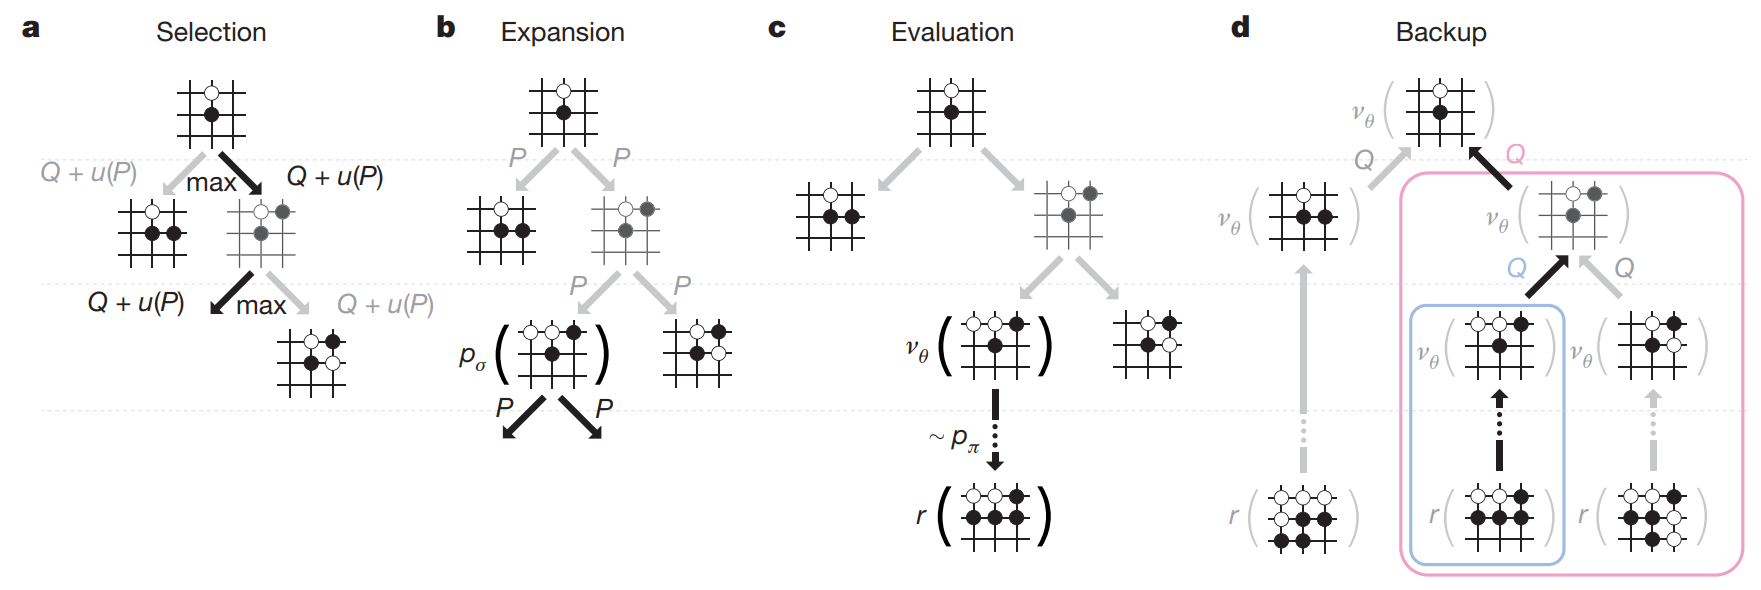
\includegraphics[scale=0.3]{./figures/AlphaGo蒙特卡洛树搜索.png}
    \caption{蒙特卡洛树搜索}
\end{figure}
AlphaGo的强化学习中动作状态价值函数$Q$是通过蒙特卡洛树搜索确定的,蒙特卡洛树搜索算法如图1所示,
搜索树的跟节点状态表示当前的状态$s$,由于搜索状态非常庞大,所以利用贪心的思想,每次优先搜索最有可能获得最高价值的路径,
并将终止状态作为搜索树的叶子节点,每次搜索完成后回溯更新动作价值函数$Q(s,a)$;但是这样贪心地搜索缺少了试探的过程,
容易陷入局部最优,所以搜索下个动作的概率还应该和访问次数成反比,具体实现见下面的详细过程解释。

设$P(s,a) = p_{\rho}(a|s)$,$N(s,a)$为动作-状态$(s,a)$的访问次数,最开始只有跟节点(当前状态)被访问到,
搜索树上仅有该一个节点,假设现在是第$n$次搜索,每次搜索均从根节点开始,蒙特卡洛搜索分为一下四步:
\begin{enumerate}
    \item 动作选择:根据动作价值函数$Q(s,a)$和一个奖励值$u(s,a)$确定选择的动作
    \begin{equation*}
        a_t = \argmax_{a}(Q(s_t,a)+u(s_t,a))
    \end{equation*}
    其中$u(s,a)\propto \frac{P(s,a)}{1+N(s,a)}$,分子$P(s,a)$就是策略网络$p_\sigma(s,a)$或$p_{\rho}(s,a)$,
    分母为该条边的访问次数,加入该项可以是的访问次数少的节点有更多的访问几率,从而模型的增强试探能力。
    \item 状态扩展:当搜索到达一个从未见过的状态节点$s_L$时(也称$s_L$为叶子节点),则需对$s_L$进行扩展,
    利用策略网络$p_{\sigma}(s,a)$或$p_{\rho}(s,a)$对$s_L$的所有合法状态$a$进行预测,得到$P(s_L,a)$。
    \item 状态评估:记$s_L$处的状态价值函数为$V(s_L)$,第一部分肯定是使用状态价值函数$v_\theta(s_L)$对其进行估计,
    第二部分则是利用最开始通过监督学习得到的简单决策网络$p_\pi(s,a)$做搜索得到的链,这条链一直搜索到终止状态,
    记最终的奖励值为$z_L$;结合上述二者确定$s_L$处的状态价值函数($\lambda$为混合因子,用于平衡两者的重要度)
    \begin{equation*}
        V(s_L) = (1-\lambda)v_\theta(s_L)+\lambda z_L
    \end{equation*}
    \item 状态回溯:在得到$s_L$的状态后,通过回溯更新$N(s,a)$和$Q(s,a)$,$N(s,a)$就是边$(s,a)$通过的累计次数,
    $Q(s,a)$则可通过强化学习理论的定义式得到
    \begin{align*}
        Q(s,a) =&\ \E[z_t|S_t=s,A_t=a] = \sum_{s_L, r}p(s_L|s,a)(r+V(s_L))\\
        \xlongequal{r=0}&\ \sum_{s_L}p(s_L|s,a)V(s_L) = \frac{1}{N(s,a)}\sum_{i=1}^n\mathrm{1}(s,a,i)V(s_L^i)
    \end{align*}
    其中$\mathrm{1}(s,a,i)$表示第$i$次搜索是否经过$(s,a)$,$V(s_L^i)$表示第$i$次搜索的叶节点。
\end{enumerate}
最后,\textbf{选择访问次数最多的动作作为当前状态的实际动作}。
\subsection{总结}
最终版本的AlphaGo分为两个版本,一个单个机器上计算40线程,48个CPU和8个GPU的小型版本;另一个是分布式版本40线程,
1202个CPU和176个GPU的大型版本。总的来说,AlphaGo做出了一下几个特点:
\begin{enumerate}
    \item 将蒙特卡洛树搜索与深度神经网络相结合,利用神经网络近似策略函数和状态价值函数,用于搜索过程中状态价值的再估计与搜索方向;
    \item 深度神经网络将有监督学习和强化学习相结合,先进行有监督学习,再在其基础上进行强化学习;
    \item 仅从与环境交互中学习,无需人工加入的特殊估值函数。
\end{enumerate}
\section{实验设计}
\subsection{实验目标}
使用论文\href{https://arxiv.org/abs/1312.5602}{Playing Atari with Deep Reinforcement Learning - 2013}中的DQN网络,
对Cartpole平衡小车问题进行求解,模型来自OpenAI在Python中的\href{https://gymnasium.farama.org/environments/classic\_control/cart\_pole/}{gymnasium库},
我通过单线程与多线程实现的方法,有效地实现了简单的DQN网络解决该问题。

Cartpole问题可以视为一个\href{https://baike.baidu.com/item/%E5%80%92%E7%AB%8B%E6%91%86/7765096}{倒立摆问题},
倒立摆是一个重心高于其\href{https://baike.baidu.com/item/%E6%9E%A2%E8%BD%B4/2010044}{枢轴}点的摆,
它是不稳定的,但是可以通过移动枢轴点位置以保持该系统的稳定性. 我们的目标是尽可能长地保持摆的垂直状态.

\begin{itemize}
    \item 紫色方块代表枢纽点.
    \item 红色和绿色箭头分别表示枢纽点可移动的水平方向.
\end{itemize}

具体的规则:一个摆通过一个无摩擦的枢轴连接到推车上,该推车沿着水平方向的无摩擦轨道移动. 
通过对推车施加 $+1$ 和 $-1$ 的推力来维持该系统平衡,保持摆的直立状态. 当杆在一个时间戳保持直立,
则获得 $+1$ 的奖励. 当杆与竖直方向的夹角超过 $15^\circ$,或者小车相对中心的移动距离超过 $2.4$ 个单位时,游戏结束.

\subsection{算法原理}
Deep Q-Learning Network (DQN)由DeepMind团队在2013年提出,论文中在多个Atari游戏中超过了人类水平,核心更新公式如下
\begin{equation*}
    Q(s_t,a_t;\bd{w}) \gets r_t + \gamma \max_{a'\in\mathcal{A}}Q(s_{t+1},a';\bd{w})
\end{equation*}
其中$Q(s,a;\bd{w})$表示网络参数为$\bd{w}$,输入为$s,a$的神经网络,输出为最优动作价值函数的估计,$\mathcal{A}$表示全部的动作集合。

在2015年在Nature上提出的论文\href{https://www.nature.com/articles/nature14236}{Human-level control through deep reinforcement learning - 2015}
中,更新公式不变,提出要在两个网络$Q(s,a;\bd{w}')$和$Q(s,a;\bd{w})$,其中$\bd{w}$为当前更新的网络,$\bd{w}'$表示之前某次的网络,
论文中说可以保持策略的稳定性,从而更容易收敛
\begin{equation*}
    Q(s_t,a_t;\bd{w}) \gets r_t + \gamma \max_{a'\in\mathcal{A}}Q(s_{t+1},a';\bd{w}')
\end{equation*}
我是按照第一篇论文实现的网络,由于问题较为简单,所以约20分钟之内能够达到最优解。
\subsection{结果分析}
下图为单线程的某次拟合效果:\href{https://imgloc.com/i/iSxhQU}{GIF动图}
\begin{figure}[H]
    \hspace{-1.3cm}
    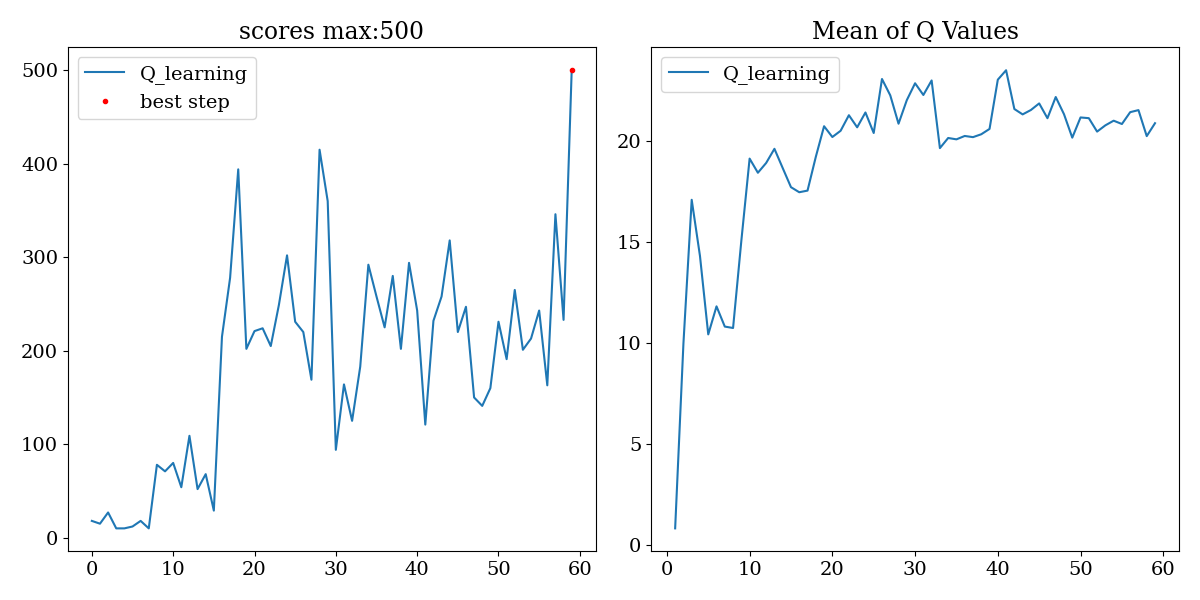
\includegraphics[scale=0.6]{./figures/Cartpole/single_process.png}
    \caption{单线程拟合效果}
\end{figure}

左侧为每幕的最优得分(达到的步数),右图为每幕下对Q值的估计。由于单线程训练样本非常少,每步之后只能对网络以大小为$32$batch对网络进行一次更新。
网络参数为:
\begin{pythoncode}
    learning_rate = 0.001
    gamma = 0.95
    BATCH_SIZE = 32
    MEMORY_SIZE = 10000
    
    EPSILON_MAX = 1.0
    EPSILON_MIN = 0.01
    EPSILON_DECAY = 0.995

    Dense1: units=32, activation="relu", type="Dense"
    Dense2: units=32, activation="relu", type="Dense"
    Output:  units=2, type="Dense"

    LOSS = MSE (Mean square of error)
    optimizer = Adam
\end{pythoncode}

下图为6线程的某次拟合效果:\href{https://imgloc.com/i/iSx9U5}{GIF动图}
\begin{figure}[H]
    \hspace{-1.3cm}
    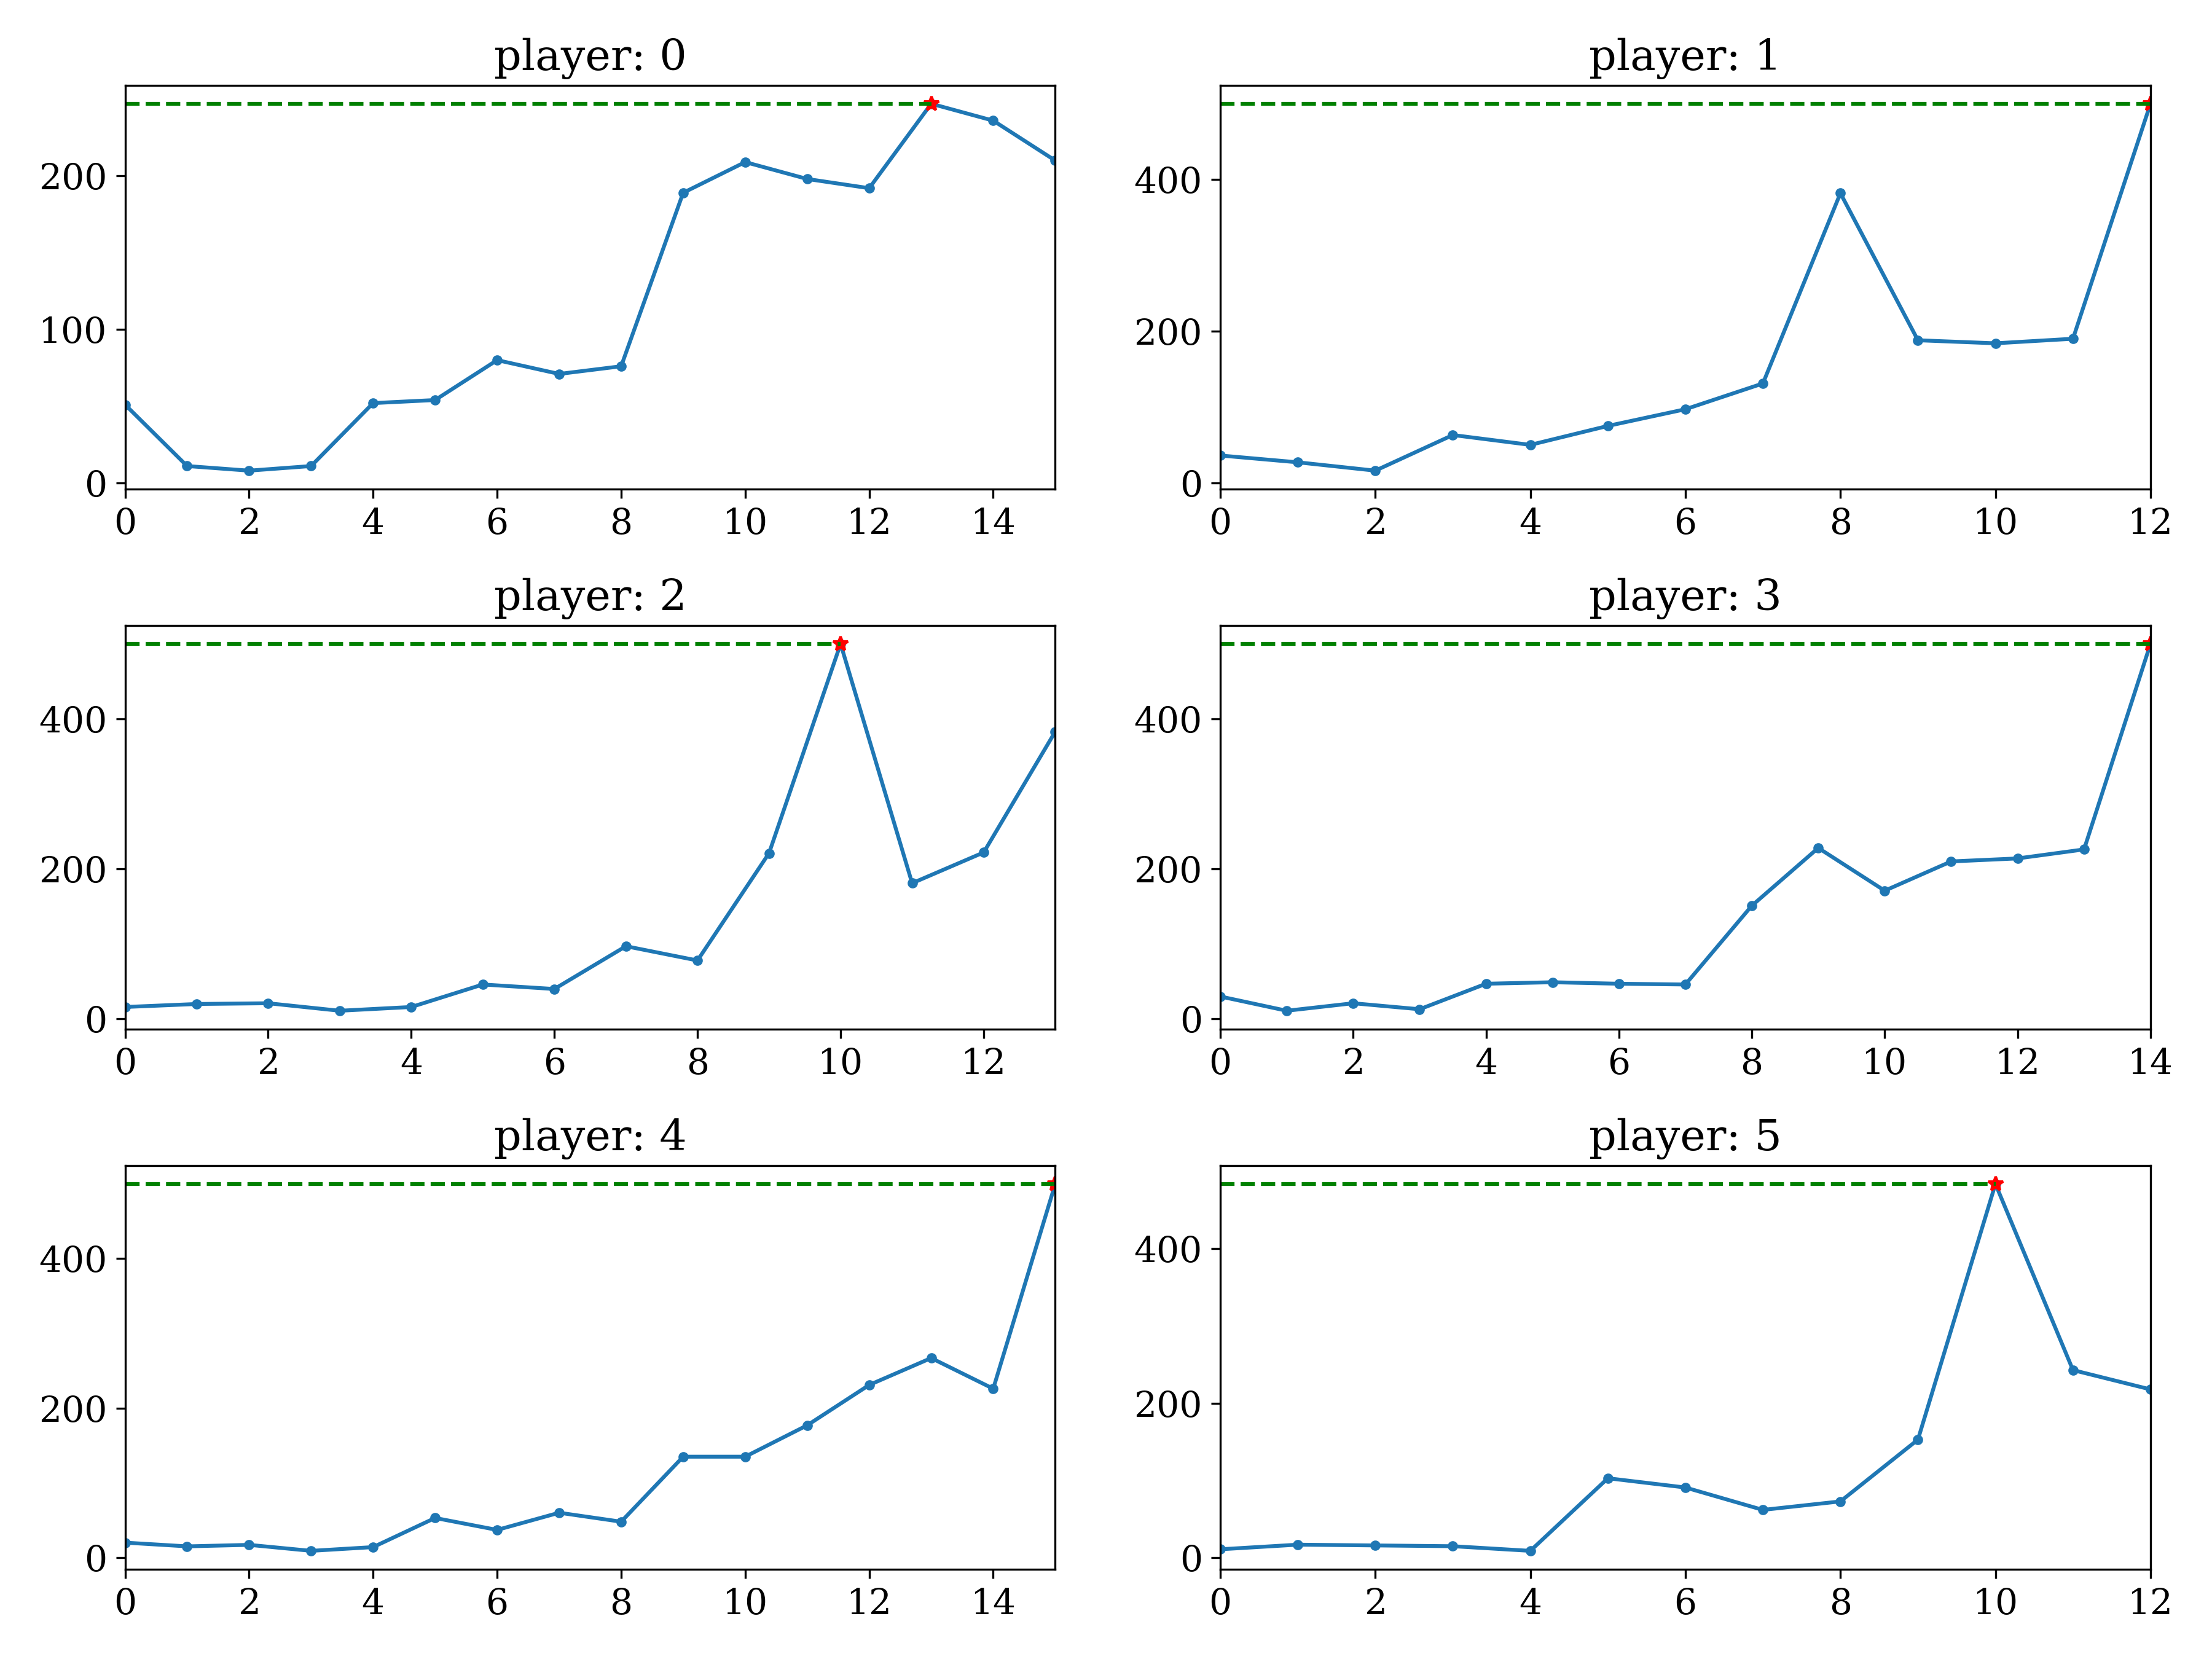
\includegraphics[scale=0.6]{figures/Cartpole/multi_process/player_logs.png}
    \caption{6个线程的拟合效果}
\end{figure}
\begin{figure}[htbp]
    \centering
    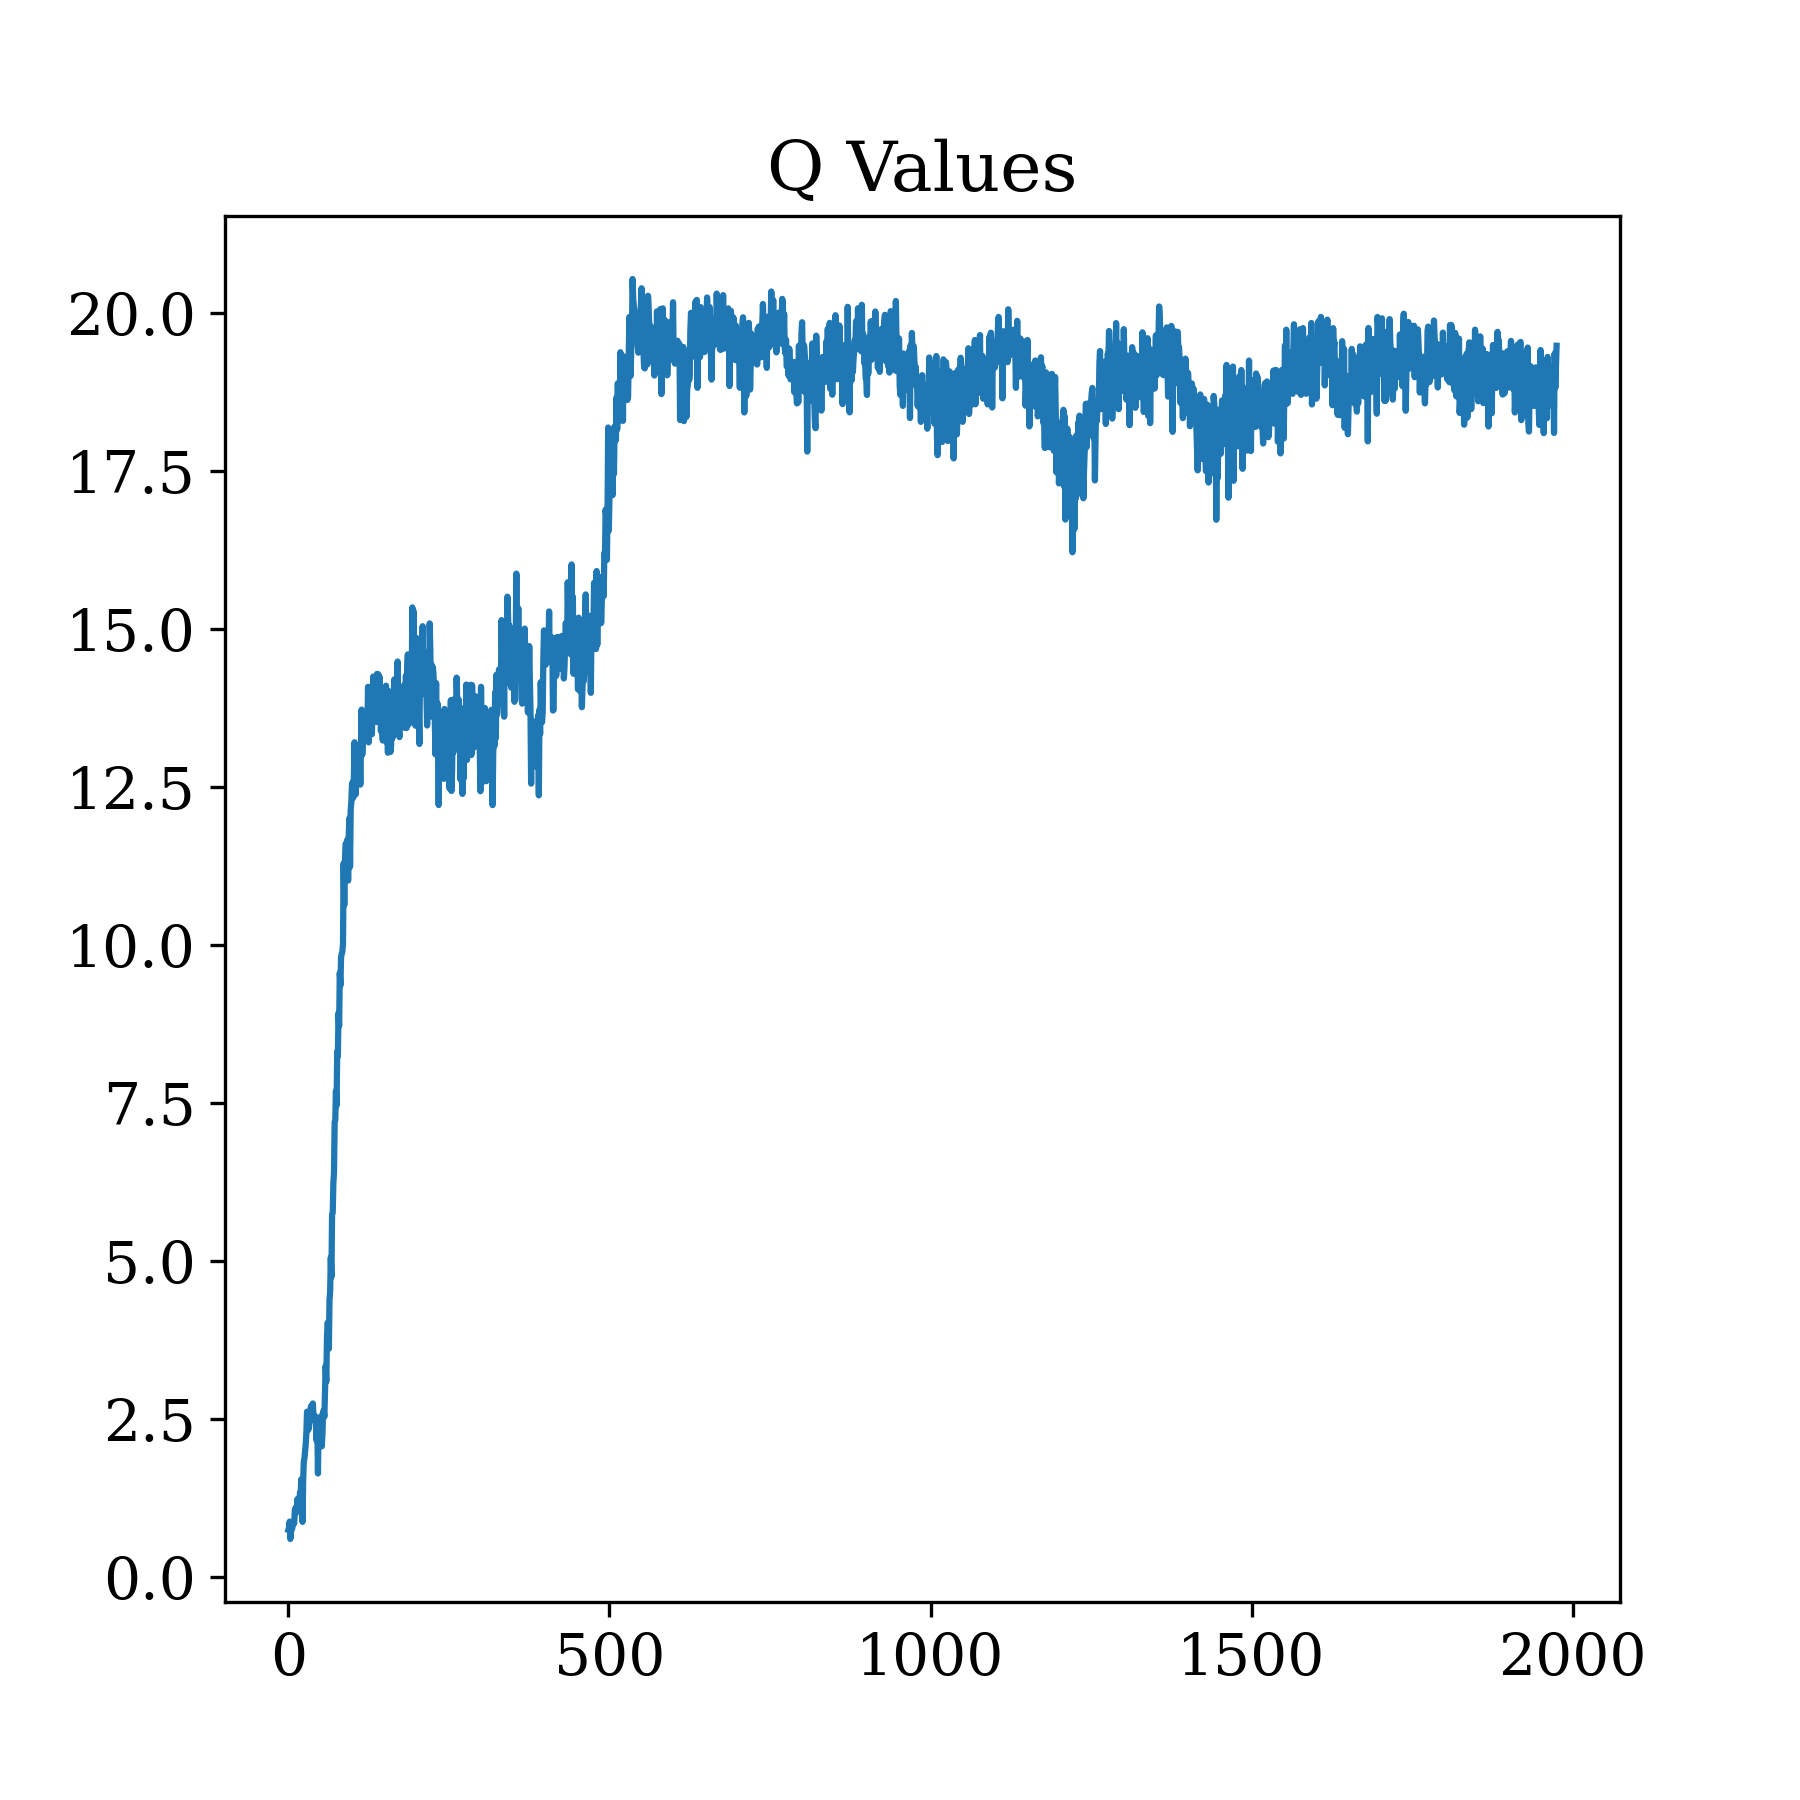
\includegraphics[scale=0.6]{figures/Cartpole/multi_process/Q_values.png}
    \caption{6线程的Q函数估计值}
\end{figure}

6线程中Q值更新更加稳定,而且训练速度更快,并且最终得到的动图中滑块移动范围更小,更加稳定,超参数与单线程相同。

具体更新的方法为统一收到6个线程返回的状态值,通过返回值传入到网络中得到每个线程的Q值估计值并记录到记忆中,并给出最优动作,
并对网络进行一次训练,每次采样的训练集大小为$6\times 32$,每个Batch大小为$32$。

\subsection{代码结构}
使用到的库版本如下:
\begin{pythoncode}
    tensorflow.__version__ = '2.12.0'  # tensorflow 2以上均可
    numpy.__version__ = '1.23.5'
    matplotlib.__version__ = '3.7.1'
    gymnasium.__version__ = '0.27.1'
\end{pythoncode}

\noindent 单线程的代码在文件夹 \texttt{code\_Catpole/single\_process}中,主要包含两个代码文件
\begin{itemize}
    \item \texttt{main.py}:单线程运行的主程序,主要由\texttt{Agent}类构成,包含数据的输入、日志保存、环境交互的功能。
    \item \texttt{dense\_net.py}:主要包含类\texttt{DenseModel},实现网络的记忆、训练与Q值预测。
\end{itemize}

\noindent 多线程的代码在文件夹 \texttt{code\_Catpole/multi\_process}中,主要包含五个代码文件
\begin{itemize}
    \item \texttt{run.py}:启动训练。
    \item \texttt{agent.py}:包含智能体\texttt{Agent}类,主要实现网络部分,具有记忆、训练与Q值预测。
    \item \texttt{player.py}:包含\texttt{Player}类,实现每个子线程的内部日志记录,独立环境创建和交互功能;\texttt{LogManager}用于处理每个\texttt{Player}类的日志,并输出到图像中。
    \item \texttt{swapper.py}:作为\texttt{Agent}与\texttt{Player}类之间的数据进行交换,开启线程池,并进行多线程操作。
    \item \texttt{constant.py}:包含全部重要超参数。
\end{itemize}

\end{document}
